\documentclass[main.tex]{subfiles}

\begin{document}
\chapter{Formation of a star from interstellar medium}
\PartialToc

\section{Broader problem of formation of a star}
(Burbidge (1960), Kahn (1960), Ebert-von Hoerner-Temesvary (1960))

Change in density from \SIrange{e-24}{1}{\gram\per\cubic\cm}

\section{Final stage of formation}
A star without neclear reactions:
\begin{itemize}
\item Optically thick system: radiation escapes only from thin surface layer
\item Hydrodynamic time-scale must be much shorter than thermal time-scale: we can calculate heat flow assuming HE.
\end{itemize}
 
\subsection{Conditions for homologous contraction}

$\TDly{\rho}{T}$: in a log-plot of temperature vs density profile during contraction every point evolve parallel to the $p_g=P_r$ line.

\chapter{Fonti energia: energia gravitazionale ed energia interna.}

A star derives its energy to shine from internal energy, thermonuclear fuel, and gravitational contraction.
\PartialToc


\section{Equilibrio meccanico locale vs constrain on star's structure}

\subsection{G-nal potential energy}
(vedi ~\ref{chap:gravity}) L'energia potentziale gravitazionale di un corpo autogravitante \'e l'opposto dell'energia necessaria per portare le masse infinitesime arbitrariamente lontane:
\begin{align*}
&d\Omega=-\int_r^{\infty}\frac{Gm(r)}{r'^2}\,dm(r)\,dr'\\
&=-\frac{Gm(r)}{r}\,dm(r)\\
&\Omega=-\int_0^M\frac{Gm(r)}{r}\,dm(r)\\
&\Omega=-q\frac{GM^2}{R}&\intertext{per densit\'a uniforme}\\
&\Omega=-\frac{3}{5}\frac{GM^2}{R}
\end{align*}

\subsection{\kh{} time-scale (sole)}
Nel caso del sole: divido l'energia potentziale G-nal per la luminosit\'a attuale
\begin{equation*}
\frac{G\msun}{\rsun}\approx\num{3.8e48}\si{\erg}/\lsun\approx\num{3e7}\,yr
\end{equation*}

\subsection{Mechanical and internal energy}

Trascuro i moti macroscopici o fenomeni turbolenti: l'energia totale di una stella

\begin{align*}
&W=\int_ME\,dm(r)+\Omega=U+\Omega\\
&U=\int_ME\,dm(r)
\end{align*}

\subsection{Equilibrium state. Adiabatic perturbation.}

Equilibrium state of the star corrisponds to extrema of $W$: hydrostatic equilibrium is an extremum relative to other configurations.

For adiabatic perturbation (abbastanza rapide da pater trascurare gli scambi di calore e abbastanza lente da poterne trascurare l'energia cinetica, adiabatic sound waves) 

\begin{align*}
&\varad{W}=0&\intertext{$\uparrow$ hydrostatic stellar equilibrium}\\
&\varad{W}=\varad{U}+\varad{\Omega}\\
&U\to U+\varad{U}=U+\delta\int_ME\,dm(r)\\
&=U+\int\delta E\,dm(r)&\intu{changes in specific internal energy of a particular mass element $dm(r)$ (Lagrangian description of the perturbation).}
\end{align*}

We label each mass element of $dm(r)$ worth of matterand see what happens to $E$ when $r$, $T$ and $\rho$ change.

\begin{align*}
&dQ=dE+P\,d\vrho{}=T\,dS&\intu{1 e 2 leggi termodinamica}\\
&\vrho=\frac{1}{\rho}
\end{align*}
Qui scrivo $\vrho{}$ per indicare il volume specifico con dimensioni \si{\cubic\cm\per\gram} cio\'e il volume associato ad 1 grammo di materia:
\begin{align*}
&\vrho{}=\frac{1}{\rho}=\frac{4\pi r^2\,dr}{dm(r)}=\frac{d(\frac{4\pi r^3}{3})}{dm(r)}\\
&\vrho{}\to\vrho{}+\var{\vrho{}}=\frac{d[4\pi\frac{(r+\var{r})^3}{3}]}{dm(r)}\vrho{}\\
&+\frac{d(4\pi r^2\var{r})}{dm(r)}&\intu{al primo ordine in $\var{r}$: $\frac{\var{r}}{r}\ll1$ and ''spherically symmetric'' perturbation.}
\end{align*}

\begin{align*}
&\varad{U}=-\int_MP\var{\vrho{}}\,dm(r)\\
&=-\int_MP\TDof{m_r}(4\pi r^2)\,dm_r\\
&\varad{U}=\int_M\TDy{m_r}{P}4\pi r^2\var{r}\,dm_r&\intu{Boundary conditions:}\\
&\var{r}(m_r=0)=0,\quad P_S=P(m_r=M)=0\\
\end{align*}

Per l'energia potenziale gravitazionale
\begin{align*}
&\Omega\to\Omega+\var{\Omega}=-\int_M\frac{Gm_r}{r+\var{r}}\,dm_r=\\
&\approx\Omega+\int_M\frac{Gm_r}{r^2}\var{r}\,dm_r
\end{align*}

\begin{align*}
&\varad{W}=\int_M[\TDy{m_r}{P}4\pi r^2+\frac{Gm_r}{r^2}]\,\var{r}\,dm_r&\intertext{condizione necessaria per l'equilibrio idrostatico:}\\
&\varad{W}=0\Leftrightarrow\TDy{m_r}{P}=-\frac{Gm_r}{4\pi r^4}&\intu{condizione di equilibrio idrostatico}
\end{align*}

\subsection{Significance of second variation of $W$}
(Cole Miller Maryland)
\begin{itemize*}
\item EOS: $P=c_1\rho\expy{\Gamma_1}$
\item write $\svarad{W}$
\item Change variable: $m_r\to V$ (terms like $\var{r}^2$ in term of $V$ and $\var{V}$)
\item if $\gamma_1$ constant throughout the star $\var{V}=kV$
\item Simplify $\svarad{W}>0$
\end{itemize*}

\section{Virial theorem}

\subsection{Virial theorem}

\begin{align*}
&\frac{1}{2}\TtwoDy{t}{I}=2K+\Omega\\
&I=\sum m_ir_i^2,\quad 2K=\sum m_iv_i^2=\sum\scap{p_i}{v_i}&\intertext{Derived for sum or integral over the whole star: if we had chosen a sphere of radius $R'<R$ the material contained within the shell $R'<r<R$ would contribute with additional term on the rhs $-3P_SV_S$ where are defined pressure at radius $R'$ and volume in same radius.}
\end{align*}


\subsection{Energia totale}

\begin{align*}
&2K=\sum m_iv_i^2=\sum\scap{p_i}{v_i}&\intu{Is it U or differs? The scala product $\scap{p_i}{v_i}$ measures the momentum transfer hence must be related to Pressure.}\\
&P=\frac{1}{3}\int n(\vec{p})\scap{v}{p}\,d^3p&\intu{$n(\vec{p})$ (dimension \si{\per\cubic\cm\per\cubic\momentum}) is the number density of particles with momentum $\vec{p}$, in the continuum limit for isotropic gas.}\\
&2K=3\int_VP\,dV\quad\Rightarrow\quad 2K=3\int_M\frac{P}{\rho}\,dm_r&\intu{ho usato che}\\
&dm_r=\rho d(\frac{4}{3}\pi r^3)\rho\,dV\\
&\frac{1}{2}\TtwoDy{t}{I}=\int_M\frac{3P}{\rho}+\Omega
\end{align*}

\subsection{$\gamma$-law equation of state}

\begin{align*}
&P=(\gamma-1)\rho E&\intertext{E is energy per uni mass (\si{\erg\per\gram}), for a monoatomic ideal gas:}\\
&\gamma=\frac{c_P}{c_V}=\frac{5}{3},\quad P=\frac{2}{3}\rho E&\intertext{for radiation or completely relativistic Fermi gas:}\\
&\gamma=\frac{4}{3},\quad K=\frac{3}{2}(\gamma-1)U&\intertext{$K=U$ only for $\gamma=\frac{5}{3}$: total kinetic energy is the same as the total internal energy only under certain circumstances ($\gamma=\frac{5}{3}$ doesn't mean necc the gas is ideal and monotonic).}
\end{align*}

Relation between W and $\Omega$ for hydrostatic stars
\begin{align*}
&\frac{1}{2}\TtwoDy{t}{I}=3(\gamma-1)U+\Omega\\
&\frac{1}{2}\TtwoDy{t}{I}=3(\gamma-1)W-(3\gamma-4)\Omega&\intertext{for hydrostatic equilibrium:}\\
&W=\frac{3\gamma-4}{3(\gamma-1)}\Omega&\intertext{hydrostatic equilibrium and dynamically stable: $W<0$ and so $\gamma>\frac{4}{3}$.}
\end{align*}

\subsection{Contracting star}

Very gradually mantaining sphericity and hydrostatic eq all time (almost)
\begin{align*}
&\Delta W=\frac{3\gamma-4}{3(\gamma-1)}\Delta\Omega&\intertext{$\gamma>\frac{4}{3}$ costante.}\\
&\Omega\propto-\frac{GM^2}{R}\Rightarrow\mvar{\Omega}\propto\frac{GM^2}{R^2}\mvar{R}&\intertext{$\mvar{\Omega}<0$ e dal viriale risulta $\mvar{W}<0$ cio\'e il sistem ha perso energia:}\\
&\mvar{U}=-\frac{1}{3(\gamma-1)}\mvar{\Omega}&\intertext{$\mvar{U}>0$ for contraction: the star heat up, the rest of energy made available by contraction $|\mvar{W}|$ is lost from the system.}
\end{align*}

For ideal gas with $\gamma=\frac{5}{3}$
\begin{equation*}
\mvar{W}=\frac{1}{2}\mvar{\Omega}=\frac{q}{2}\frac{GM^2}{R^2}\mvar{R}
\end{equation*}

Ipotiziamo che la variazione di energia totale per unit\'a di tempo sia uguale in valore assoluto uguale alla luminosit\'a della stella
\begin{align*}
&L=-\TDy{t}{W}=-\frac{q}{2}\frac{GM^2}{R}(\frac{1}{R}\TDy{t}{R})&\intertext{If L is constant we have an e-folding time:}\\
&\tkh{}\approx\frac{q}{2}\frac{GM^2}{LR}\\
&\tkh{}(q\approx\frac{3}{2})\\
&\approx\num{2e7}(\frac{M}{\msun{}})^2(\frac{L}{\lsun{}})\expy{-1}(\frac{R}{\rsun{}})\expy{-1}\,yr&\intertext{this q value is representative for the sun}
\end{align*}

\section{Gravitational energy generation rate}

\subsection{Thermal balance}

For a given \si{\gram} of material the local rate of thermonuclear energy generation is balanced by mass divergenge of luminosity
\begin{equation*}
\PDy{m_r}{l_r}=\epsilon,\quad [\epsilon]=\si{\erg\per\gram\per\second}
\end{equation*}

If the equality doesn't hold the energy content varies
\begin{align*}
&\TDy{t}{Q}=\PDy{t}{E}+P\PDof{t}(\frac{1}{\rho})=\epsilon-\PDy{m_r}{l_r}&\intertext{$Q$ is the heat content in \si{\erg\per\gram} (Lagrangian mode: a particular gram of matter is followed in time).}\\
&\PDy{m_r}{l_r}=\epsilon+\epsilon_g\\
&\epsilon_{g}=-[\PDy{t}{E}+P\PDof{t}(\frac{1}{\rho})]\\
&\epsilon_g=-\frac{P}{\rho(\Gamma_3-1)[\PDy{t}{\ln{P}}-\Gamma_1\PDy{t}{\ln{\rho}}]}&\intu{for $\Gamma_1$ constant in time: vedi \cite{cox68stellar} $\S 17.6$.}\\
&\epsilon_g=-\frac{P}{\rho(\Gamma_3-1)}\PDof{t}[\ln{\frac{P}{\rho\expy{\Gamma_1}}}]
\end{align*}

\subsection{Departures from adiabaticity}

$\epsilon_g=0$ for adiabatic process where $P\propto\rho\expy{\Gamma_1}$: energy release in gravitational sources arises from departures from adiabaticity during contraction or expansion. If the pressure rises less than adiabatic upon compression $P\propto\rho\expy{\Gamma_1-\delta}$ then $\epsilon_g=\delta\frac{P}{\rho(\Gamma_3-1)}\PDy{t}{\ln{\rho}}>0$: a less than adiabatic rise of pressure upon compression implies that energy is being released by $P\,dV$ work ($dq=du+P\,dV$).


\chapter{Modelli Stellari.}
\PartialToc

\section{Teorema Vogt-Russel}

In those cases where VR theorem is not valid (where specification of M and chemical composition fails to determine a model uniquely) some information about star's evolution history are needed.

\subsection{Usefull rule of thumb}

Complete structure of a star in hydrostatic and thermal equilibrium is uniquely determined by total mass and run of chemical composition throughout the star: provided pressure, internal energy per unit mass, opacity, and energy generation rate are functions only of density, temperature and chemical composition.

\subsection{Order of magnitude estimates: theoretical relation between fundamental parameter.}

Let us consider a star of mass M and radius R in HE:
\begin{align*}
&\rho=\frac{M}{R^3}\\
&P\approx G\frac{M^2}{R^4}&\intertext{internal pressure must be great enough to support weight of overlying layers,}\\
&T=\frac{\mu}{\gasconstant{}}\frac{P}{\rho}\approx\frac{G}{\gasconstant{}}\frac{\mu M}{R}&\intertext{specification of equation of state further determine T. There is an energy outflow: for a given temperature gradient the luminosity is determined by opacity (assuming radiative transport), in diffusion approximation:}\\
&\TDof{r}(\frac{1}{3}aT^4)=-\frac{\kappa\rho}{c}\frac{l}{4\pi r^2}\\
&L_{rad}\approx\frac{4\pi ac}{3}R^2\frac{T^4}{R}\frac{1}{\kappa\rho}=\frac{4\pi ac}{3}R\frac{T^4}{\kappa\rho}\\
&=\frac{4\pi ac}{3}(\frac{G}{\gasconstant{}})^4\frac{\mu^4M^3}{\kappa}&\intertext{Per l'opacit\'a introduco la legge di Kramer:}\\
&\kappa=\kappa_0\rho T\expy{-3.5}\\
&=\kappa_0(\frac{\gasconstant{}}{G})\expy{3.5}\frac{R\expy{0.5}}{\mu\expy{3.5}M\expy{2.5}}
\end{align*}

\begin{usefull}{Mass-Luminosity law (theoretical)}
\begin{align*}
&L_{rad}=\frac{4\pi ac}{3}(\frac{G}{\gasconstant{}})^4\frac{\mu^4M^3}{\kappa}&\intu{appropriate for constant opacity (Thomson scattering by free electron)}\\
&L_{rad}=\frac{4\pi ac}{3\kappa_0}(\frac{G}{\gasconstant{}})\expy{7.5}\frac{\mu\expy{7.5}M\expy{5.5}}{R\expy{0.5}}&\intertext{appropriate for Kramer's opacity law}
\end{align*}

\end{usefull}


L is determined only by M and chemical composition ($\mu$, $\kappa_0$) and weakly by R. Nuclear energy sources influence mass distribution but usually is a small effect.

\begin{usefull}{Radius-$L_{nucl}$ relation}
Now we use the condititon of thermal equilibrium
\begin{align*}
&L_{gen}=\int_0^M\epsilon\,dm\approx\epsilon M&\intertext{for a star burning hydrog via carbon cycle}\\
&\epsilon=\epsilon\rho T\expy{17}\\
&L_{gen}\approx\epsilon_0(\frac{G}{\gasconstant{}})\expy{17}\frac{\mu\expy{17}M\expy{19}}{R\expy{20}}
\end{align*}
\end{usefull}

The condition of thermal equilibrium $L_{gen}=L_{rad}$ uniquely determines R for given chemical composition and mass.


\section{Modello omogeneo in equilibrio}

Treatment of homologous stars using dimensional analysis.

\subsection{Homologous stars}

Sequences of stellar models in complete equilibrium where one is related to the other by a simple change in scale: all have the same constituent physics, the same uniform composition and that, chosen a reference in the sequences indicated with $0$ subscript
\begin{align*}
&r=\frac{R}{R_0}r_0\\
&m_r=\frac{M}{M_0}m_{r0}
\end{align*}

\subsection{Energy generation/transport: power law constitutive equations.}

Indico la produzione di energia per grammo in un guscio sferico $dm_r$ e spessore $dr$ con $\epsilon$ (\si{\erg\per\second\per\gram}).
\begin{align*}
&l(r+\,dr)-l(r)=dl(r)=4\pi r^2\rho\epsilon\,dr=\epsilon\,dm(r)\\
&\PDy{r}{l(r)}=4\pi\rho r^2\epsilon,\quad\TDy{l_r}{m_r}=\epsilon&\intertext{Thermal balance, energy equation}
\end{align*}

Power law for $\epsilon$
\begin{align*}
&\epsilon=\epsilon_0\rho\expy{\lambda}T\expy{\nu}\\
&\lambda=1,\quad \nu\approx4&\intertext{pp-chains}\\
&\lambda=1,\quad \nu\approx15&\intertext{CNO cycles}\\
&\lambda=2,\quad \nu\approx40&\intertext{Triple-$\alpha$}
\end{align*}

In the interior of the stars the energy flux obey to Fick's law of diffusion $F(r)=-D\TDy{r}{(aT)^4}$
\begin{align*}
&l(r)=-\frac{4\pi r^2c}{3\kappa\rho}\TDy{r}{aT^4}\\
&l_r=-\frac{(4\pi r^2)^2c}{3\kappa}\TDy{m_r}{aT^4}\\
&\kappa=\kappa_0\rho^nT\expy{-s}\si{\square\cm\per\gram}
\end{align*}

\subsection{Stellar dimensional analysis}
Simple treatment  of homologous stars using dimensional analysis 

\begin{align*}
&P\propto\frac{M^2}{R^4}&\intertext{Lagrangian form hydrostatic equilibrium}\\
&P_0=\rho\expy{\chi_{\rho}}T\expy{\chi_T}\\
&d\ln{P}=\chi_{\rho}\,d\ln{\rho}+\chi_T\,d\ln{T}&\intertext{$\chi_{\rho}$ and $\chi_T$ are assumed to be the same for all the stars in the collection.}
\end{align*}

\subsection{Energy, hydrostatic, diffusive radiative, constitutive equations: power law.}

\begin{align*}
&R\propto M^{\alpha_R}\\
&\rho\propto M^{\alpha_{\rho}}\\
&T\propto M^{\alpha_T}\\
&L\propto M^{\alpha_L}
\end{align*}

We insert the above relations in the equilibrium equation in differential form

\subsubsection{Radiative energy transfer}
\begin{align*}
&
\begin{pmatrix}
3&1&0&0\\
4&\chi_{\rho}&0&\chi_T\\
0&\lambda&-1&\nu\\
4&-n&-1&4+s\\
\end{pmatrix}
\begin{pmatrix}
\alpha_R\\
\alpha_{\rho}\\
\alpha_L\\
\alpha_T\\
\end{pmatrix}
=\begin{pmatrix}
1\\2\\-1\\1\\
\end{pmatrix}
\end{align*}

The solutions are
\begin{align*}
&\alpha_R=\frac{1}{3}[1-2\frac{\chi_T+\nu-s-4}{D_{rad}}]\\
&\alpha_{\rho}=2\frac{\chi_T+\nu-s-4}{D_{rad}}\\
&\alpha_L=1+2\frac{2\lambda(\chi_T+\nu-s-4)-2\nu(\chi_{\rho}+\lambda+n)}{D_{rad}}\\
&\alpha_T=-2\frac{\chi_{\rho}+\lambda+n}{D_{rad}}
\end{align*}

\subsubsection{Convective energy transfer}

If energy transport is convective we can use (altough the result are of limited use)
\begin{align*}
&T(r)\propto\rho(r)\expy{\Gamma_3-1}\\
&\Gamma_3-1=\Dcad{\TDly{\rho}{T}}
\end{align*}

quindi
\begin{align*}
&
\begin{pmatrix}
3&1&0&0\\
4&\chi_{\rho}&0&\chi_T\\
0&\lambda&-1&\nu\\
0&\Gamma_3-1&0&-1\\
\end{pmatrix}
\begin{pmatrix}
\alpha_R\\
\alpha_{\rho}\\
\alpha_L\\
\alpha_T\\
\end{pmatrix}
=\begin{pmatrix}
1\\2\\-1\\1\\
\end{pmatrix}
\end{align*}


\subsection{Sequenza principale. Relazioni semi-empiriche.}
The stars we think we know the most about are located on the hydrogen main sequence.

\subsubsection{Massive stars}
The stars on the upper massive luminous part of main sequence have higher central temperature

The opacity is determined by electron scattering so $n=s=0$. The energy is generated by CNO cycle so $\lambda=1$, $\nu\approx15$.
Radiative transport of energy dominates the outer part and pressure is largely determined by ideal gas law for which $\chi_{\rho}=\chi_T=1$. Confronto fit dati osservativi/equazioni stelle omologhe (the Sun appears as reference in the homologous set of stars.)
\begin{align*}
&\alpha_R=0.78,\quad\alpha_L=3.0&\intu{exponent calculated using  homologous relations,}\\
&\frac{R}{\rsun{}}\approx(\frac{M}{\msun})\expy{0.75},\quad\frac{L}{\lsun{}}\approx(\frac{M}{\msun{}})\expy{3.5}&\intu{data fit for stellar mass greater than few solar masses;}\\
&\alpha_T=0.22,\quad\alpha_{\rho}=-1.33&\intu{in upper main sequence T should increses with mass whereas density should decrese.}
\end{align*}

\subsubsection{Lower MS (Less Massive stars)}
Is more difficult to treat. The pp-chain dominate energy generation and Kramer's opacity operates for much of the star, convection is important especially for low mass stars. Structure of these stars is determined by what happens at very outermost radiative surface.

Empirically result $\alpha_L\approx3.9$ where the homologous equations predict 5.5.


\section{Modello standard del sole}

\subsection{Il sole.}

\begin{align*}
&\msun=2*10^{33}gr\\
&\text{Age}=4.55*10^9\,yr\\
&\rsun=7*10^5 Km\\
&\tsunc=1.57*10^7 K\\
&\tsuns=6*10^3 K\\
&\rhosunc=130gr/cm^3\\
&\lsun=3.8*10^{26}W=3.8*10^{33}erg/s\\
&\Phi_{\nu}(\Pproton\Pproton)=6.0*10^{10}cm^{-2}s^{-1}\\
&\Phi_{\nu}(^8B\to^8Be^*+\APelectron+\Pnue)=6.0*10^6cm^{-2}s^{-1}\\
&X=74\%,\,Y=23,\,Z=3&\intertext{$\uparrow$ Attuale}\\
&X=75\%,\,Y=22,\,Z=3&\intertext{$\uparrow$ Composizione iniziale}\\
\end{align*}

\subsection{Equilibrio idrostatico.}
\begin{align*}
&dS\,(P(r)-P(r+\,dr)-F_g(r))=0\\
&F_g(r)=G\frac{m(r)\rho(r)\,dV}{r^2}&\intertext{se ho simmetria sferica}\\
&\frac{dm}{dr}=4\pi\rho(r)r^2
\end{align*}

Posso trascurare la BE gravitazionale?
\begin{align*}
&B_{\odot}=N_Pm_p-\msun=-E_G=\frac{3}{5G\frac{\msun^2}{\rsun}}\\
&\approx10^{-6}\msun c^2
\end{align*}

\subsection{Equazione di stato.}

\begin{align*}
&P=P(\rho,T,X,Y,Z)=P_{Gas}+P_{Rad}&\intertext{Gas ideale}\\
&P_{Gas}=K\rho T\\
&P_{Rad}=\frac{1}{3}aT^4
\end{align*}

\subsection{Produzione di energia}
\begin{align*}
\epsilon=\frac{\text{Energia prodotta}}{\text{Massa}*\text{Tempo}}&\intertext{L'energia prodotta per fusione}\\
\epsilon=\epsilon_F(\exv{\sigma v},\rho,T,X,Y,Z)&\intertext{\'e legata alla luminosita tramite}\\
\frac{d\lu}{dr}=\epsilon_F(r)4\pi r^2
\end{align*}

\subsection{Reaction Rate}
La radiazione che raggiunge la terra ha un flusso di $1.4*10^3 W/m^2$ quindi la potenza irraggiata \'e $4*10^{26} W$: dato che ogni reazione di fusione libera 25 MeV sono necessarie $10^{38} \text{Fusioni}/sec$ (4 $^1H$ per fusione).

\begin{equation*}
N_{Reaz}=\frac{\exv{R_{PP}}}{n_P}N_p(core)
\end{equation*}

\subsection{Flusso neutrini}
\begin{equation*}
\Phi_{\nu}=\frac{\dot{N_{\nu}}}{4\pi d^2}=7*10^{10}\frac{\Pnu}{s*cm^2}
\end{equation*}



\chapter{Modello stellare. Fasi evoluzione stellare.}
\PartialToc

\section{Modellizzazione stellare rappresentata nel diagramma di \hr{}.}


\subsection{Subdwarf}

\begin{figure}[!ht]
\centering
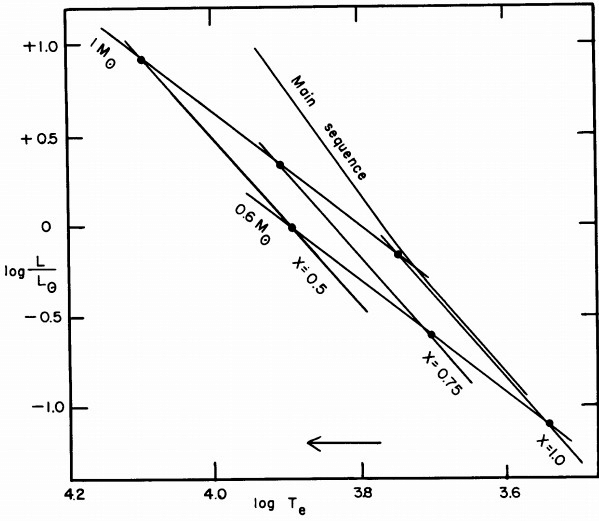
\includegraphics[width=(0.99\textwidth),height=(\textheight),keepaspectratio]{subdwarfHR}
\caption{\hr{} diagram of sub dwarf model.}
\end{figure}

\begin{figure}[!ht]
\centering
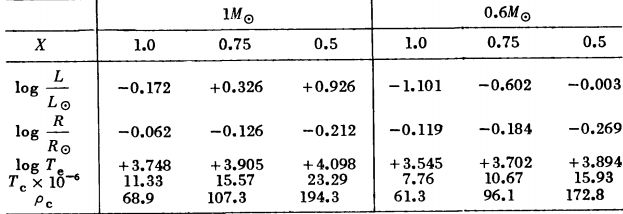
\includegraphics[width=(0.99\textwidth),height=(\textheight),keepaspectratio]{subdwarftable}
\caption{Characteristic of $0.6\msun{}$ and $1\msun{}$ sub dwarf model.}
\end{figure}

\clearpage

\subsection{Main sequence}

\begin{figure}[!ht]
\centering
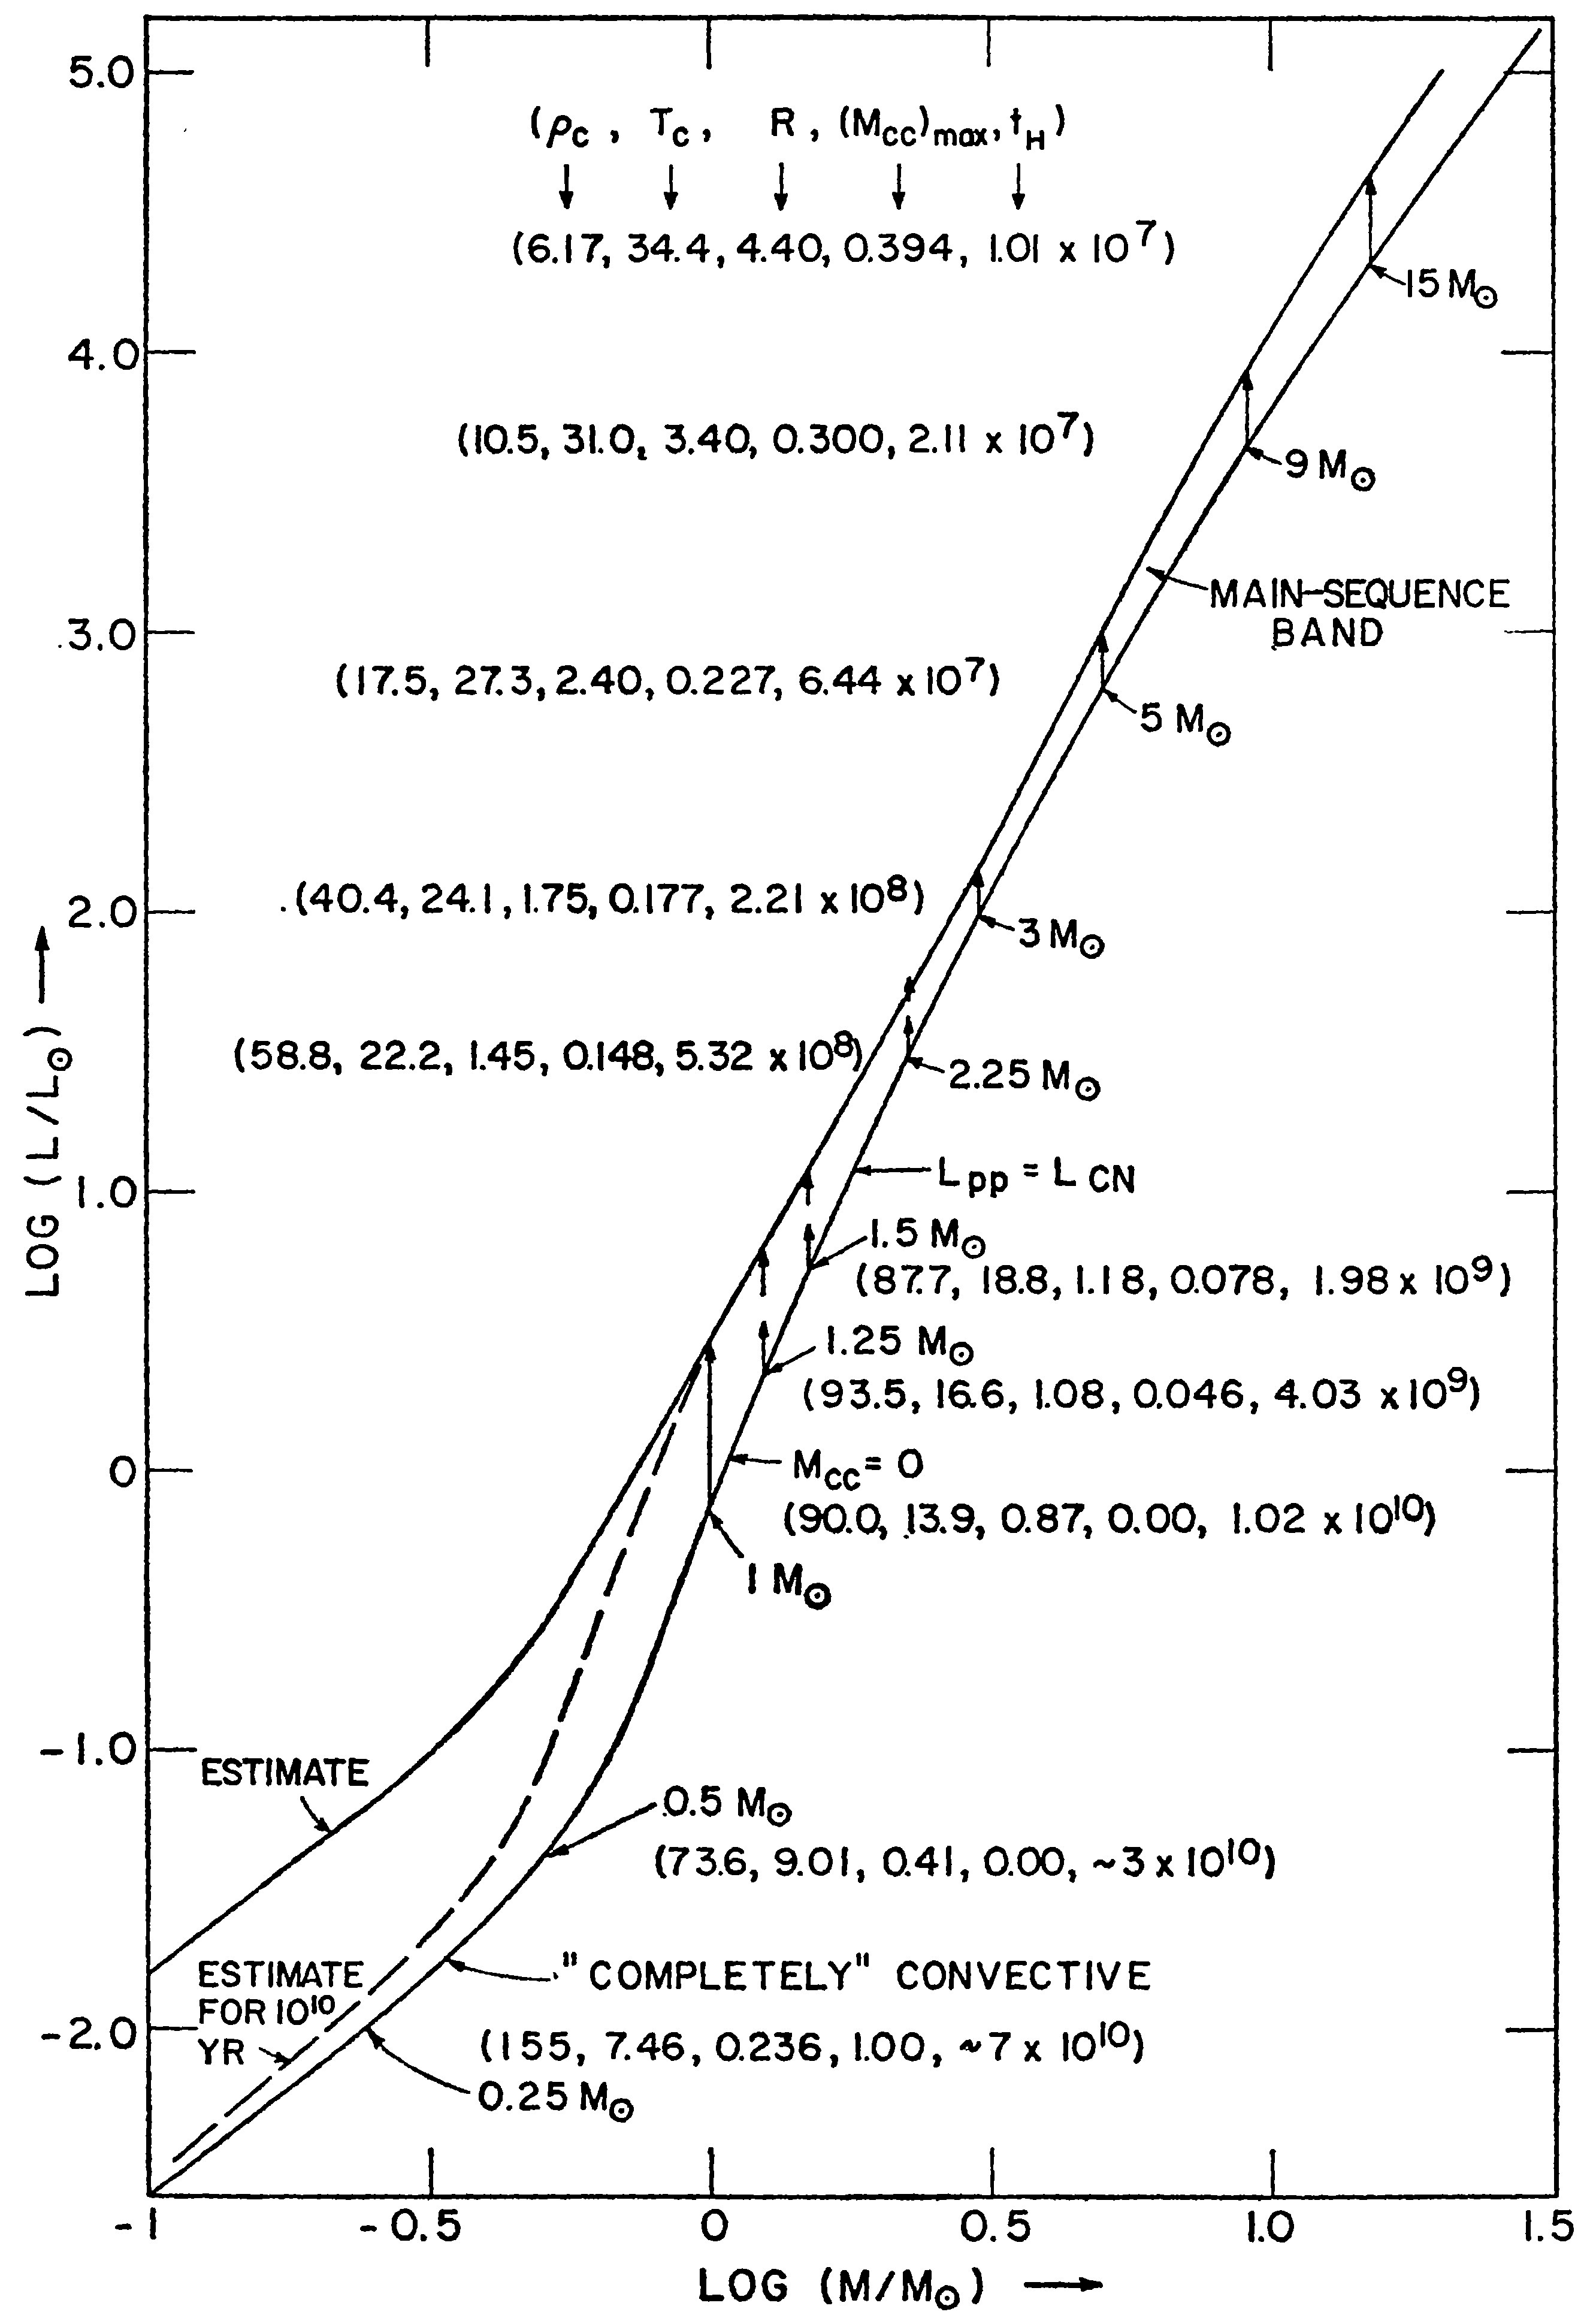
\includegraphics[width=(0.99\textwidth),height=(0.9\textheight),keepaspectratio]{MSband}
\caption{Position in M-L diagram during MS for metal rich stars. L and M are in solar units. Lower curve defines locus of homogeneous initial MS model. Number in parenthesys are \mblock{(\rho,T_6,R,\frac{M_{conv-core}^{Max}}{M},\tau_{MS})}}
\end{figure}


\clearpage

\subsection{Stellar evolution}

\begin{figure}[!ht]
\centering
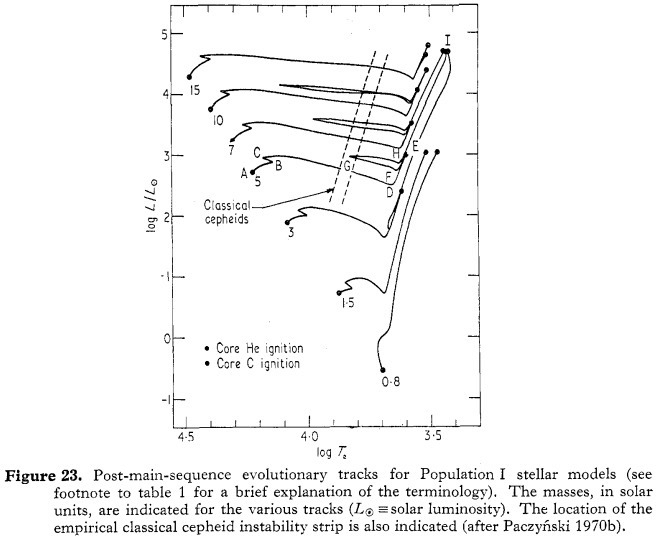
\includegraphics[width=(0.99\textwidth),height=(\textheight),keepaspectratio]{PMSevotrack}
\caption{Post MS track for population I stellar models.}
\end{figure}


\begin{figure}[!ht]
\centering
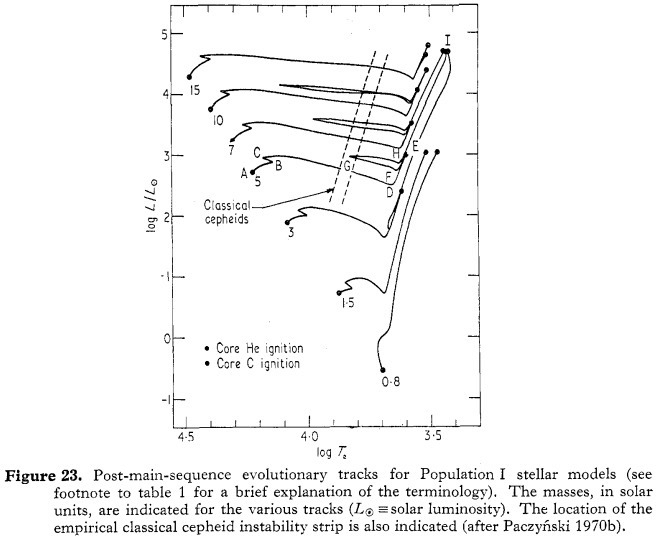
\includegraphics[width=(0.99\textwidth),height=(\textheight),keepaspectratio]{PMSevotrack}
\caption{Post MS track for population I stellar models.}
\end{figure}
ETlowmass
fiveMsunevo
evolutionMvar
timeMvar
PMSevotrack
\clearpage

\section{Composizione chimica.}

\subsection{Metallicit\'a.}
L'assenza di fusione negli strati superficiali delle stelle da dove si originano le righe fa supporre  che la loro composizione sia quella iniziale, a parte fenomeni di dredge up e sedimentazione.

La somma degli elementi pi\'u pesanti di He cresce passando da Pop. II a Pop. I.

\subsection{Formazione iniziale di metalli.}

Modelli cosmologici prevedono $Z_{in}<\num{e-6}$ mentre le stelle pi\'u vecchie osservate mostrano Z maggiore di circa 3 ordini di grandezza.

\subsection{Nucleosintesi.}
Primordial elements: they carry cosmological informations.

Prima ipotesi: decadimento di $\Pneutron\to\Pproton$ would initiates chain of neutron captures.

Von Weizsacker: nucleosynthesis in the context of stars evolutions.

Primordial fire-ball may have produced many of lightest elements but most of those with nuclear charge $Z\geq6$ are ashes of nuclear burning during stellar evolution.

Heavy elements in extreme pop II object are less abundant compared to H than they are in pop I by a factor $>100$.

He is absent in extreme popII stars.

\subsection{Galaxy chemical composition.}

If no concentration mechanism exists than the galaxy has synthetized $99\%$ of its own heavy elements.

If galaxy formed with significant abundance of He and rare elements ($D\indices{^2},He\indices{^3},Be\indices{},B\indices{}$) it must be interpreted as residual of earlier history.

\subsection{Synthesis at stellar surface.}

Non-thermal events: spallation of heavier nuclei by energetic flare particles or shock phenomena in supernovae envelopes.

\subsection{Produced in early phase of stars formations.}


\section{Fasi finali dell'evoluzione stellare.}

\subsection{Teorema del viriale}
Relazione tra l'energia cinetica media e l'energia potenziale di un sistema in equlibrio stabile o quasi-stabile.

\begin{align*}
&G=\sum_i\scap{p_i}{r_i}=\frac{1}{2}(\sum_im_ir_i^2)^2=\frac{1}{2}\frac{dI}{dt}&\intertext{I momento d'inerzia}\\
&\frac{dG}{dt}=\sum_i\scap{\dot{r_i}}{p_i}+\sum_i\scap{r_i}{\dot{p_i}}=2T\\
&+\sum_i\scap{r_i}{f_i}&\intertext{l'ultimo termi del membro di destra \'e il  viriale di Clausius}\\
&\intertext{Assumendo che la forza tra le particelle segua una legge di potenza della distanza con esponente n(del potenziale) e sia derivabile da un potenziale}\\
&\frac{dG}{dt}=2T-n\mathcal{U}&\intertext{dove U \'e l'energia potenziale totale del sistema}\\
&\frac{dG}{dt}=\frac{1}{2}\frac{d^2I}{dt^2}=2T+\Omega&\intertext{per il potenziale gravitazionale n=-1}\\
&2\overline{T}+\overline{\Omega}=0&\intertext{se il sistema \'e periodico la media del lato sinistro su un periodo dell'equazione sopra \'e nullo}
\end{align*}

\subsection{Fasi di contrazioni ed espansioni successive.}

Terminato l'idrogeno il core di elio si contrae non essendoci pi\'u fonti di energia fino a che si raggiungono T sufficienti per la fusione di dell'elio.

Detti m massa del core e r suo raggio
\begin{align*}
&E_G=-G\frac{m^2}{r}&\intertext{quindi in fase di contrazione}\\
&\Delta E_G=\frac{Gm}{r^2}\Delta r<0&\intertext{da cui risulta aumento di energia cinetica}\\
&\Delta E=-\frac{1}{2}\Delta U_G>0
\end{align*}

\subsection{fase di fusione dell'elio ($T\approx10^8K$).}

Fusione di elio-4 in carbonio-12
\begin{align*}
&^4He+^4He\to ^8_4Be\quad(\tau\approx10^{-16}s)\\
&^8Be+^4He\to^{12}C+\gamma&\intertext{al crescere di T}\\
&^{12}C+^4He\to ^{16}O+\gamma\\
&^{16}O+^4He\to^{20}Ne+\gamma
\end{align*}

\subsection{Fase di fusione del carbonio-12.}

\begin{align*}
^{12}C+^{12}C&\to ^{16}O+2^4He\\
&\to ^{20}Ne+^4He\\
&\to ^{23}Na+\Pproton\\
&\to^{24}Mg+\gamma
\end{align*}

\subsection{Fase fusione Ossigeno.}
\begin{align*}
^{16}O+^{16}O&\to ^{28}_{14}Si+^4He\\
&\to^{31}_{15}P+\Pproton\\
&\to ^{32}S+\gamma
\end{align*}

e cos\'i via fino al $^{56}Fe$ per le stelle pi\'u massicce.

\subsection{Destino finale della stella}

\begin{itemize*}
\item $M<8\msun$: Nane bianche ($R\approx R_T$).
La pressione di degenerazione degli elettroni blocca il collasso.

\item $8\msun<M<25\msun$: stella di neutroni.
La nucleosintesi raggiunge il $^{56}Fe$  poi hanno luogo fenomeni di cattura elettronica (neutronizzazione della materia): sintesi elementi pi\'u pesanti.

\item $M>25\msun$: buco nero.

\end{itemize*}


\chapter{Modelli di Stelle politropi}
\PartialToc.


\section{Polytropic gaseous spheres}

\subsection{Polytropic changes.}

\begin{definition}{Polytropic changes.}
Un elemento di materia subisce una trasformazione politropica se $dQ=cdT$ con c costante o pi\'u in generale se durante il processo di stirring la quantit\'a di calore $dQ$ fornita \'e proporzionale alla variazione istantanea di temperatura.

\begin{align*}
&(c_v-c)\,dT+P\,dV=0\\
&(c_V-c)\frac{dT}{T}+(c_p-c_V)\frac{dV}{V}=0\\
&P=K\rho\expy{\gamma'}\\
&\gamma'=\frac{c_P-c}{c_V-c}\\
&(n=-\frac{v\,dp}{p\,dv})\\
&\rho=\lambda\theta^n
\end{align*}

\end{definition}

\subsection{Limitation on stellar structure from hydrostatic equilibrium}

Impongo una relazione fra pressione e densit\'a che \'e un'idealizzazione di certe condizioni fisiche: \'e possibile separare la parte meccanica da quella termo-energetica.

\begin{align*}
&\nabla^2\Phi=4\pi G\rho&\intertext{$\uparrow$ il potenziale gravitazionale \'e soluzione dell'equazione di Poisson, che per simmetria sferica diventa:}\\
&\frac{1}{r^2}\frac{d}{dr}(r^2\frac{d\Phi}{dr})=4\pi G\rho\\
&\frac{dP}{dr}=-\frac{d\Phi}{dr}\rho=-g(r)\rho=\frac{Gm(r)}{r^2}\rho&\intertext{
Se la densit\'a non dipende dalla temperatura sostituisco la relazione $P(\rho)$ nelle equazioni meccaniche $\uparrow$}
\end{align*}

Assumo che esista una relazione del tipo
\begin{align*}
&P=K\rho^{\gamma}=K\rho^{\frac{n+1}{n}}&\intertext{ho una relazione politropa di ordine n}\\
&n=\frac{1}{\gamma-1}
\end{align*}

\subsection{Properties of solutions}

The Lane-Emden equation has a regular singularity at $z=0$:

\begin{align*}
&w(z)=1+a_1z+a_2z^2+\ldots &\intertext{con}\\
&a_1=w'(0),\quad 2a_2=w''(0),\quad\ldots &\intertext{ $a_1=0$ dato che $|\vec{g}|=\frac{d\Phi}{dr}\propto\frac{dw}{dz}$. Inserendo nell'equazione di Lane-Emden e confrontando}\\
&w(z)=1-\frac{1}{6}z^2+\frac{n}{120}z^4+\ldots &\intertext{It can be shown that for $n<5$ the radius polytropic models is finite, otherwise is infinite.}
\end{align*}

For $n<5$ the integration comes to a point where $w(z)=0$ ie $\rho=0$: the value of z, which correspons to the surface of polytrope, grows monotonically with index $n$.

One can use solution with singularity at the center for outer part of the star.

\subsection{Isothermal ideal gas.}

\begin{align*}
&\rho=\frac{\mu P}{RT}&\intertext{Per una stella isoterma di temperatura $T_0$ l'equazione di stato pu\'o essere scritta in forma di politropa }\\
&K=\frac{RT_0}{\mu}\\
&\gamma=1,\quad n=\infty
\end{align*}

\subsection{Completely convective star (Kelvin)}

Adiabatic convective equilibrium: any mass element doing convective motion is at same $T$ and $\rho$ of the surrounding.

\begin{align*}
&\nabla=(\frac{d\ln{T}}{d\ln{P}})_{ad}=\nabla_{ad}&\intertext{Per un gas completamente ionizzato e pressione di radiazione trascurabile}\\
&\nabla_{ad}=\frac{2}{5}\quad\Rightarrow\quad T\propto P^{\frac{2}{5}}&\intertext{dato che per un gas ideale con $\mu$ costante vale $T\propto\frac{P}{\rho}$ ho}\\
&P\propto\rho^{\frac{5}{3}},\quad n=\frac{3}{2}
\end{align*}

\subsection{Homogenous star}

\begin{align*}
&\rho=K_1P^{\frac{1}{\gamma}},\quad\gamma=\infty
\end{align*}

\subsection{Equazione di Lane-Emden: relazione politropica e equilibrio idrostatico.}

Hydrostatic equilibrium
\begin{equation*}
\TDy{r}{P}=-\TDy{r}{\Phi}\rho,\ (\vec{g}=-\nabla\Phi)
\end{equation*}

\begin{align*}
&\rho=\lambda\Phi^n&\intertext{Motivated by the fact that in a non degenerate polytrope of index n $\rho\propto T^n$}
&\frac{d\Phi}{dr}=-\gamma K\rho^{\gamma-2}\frac{d\rho}{dr}&\intertext{per $\gamma\neq1$ integro $\uparrow$:}\\
&\rho=(\frac{-\Phi}{(n+1)K})^n&\intertext{e sostituendo nel lato destro dell'equazione di Poisson ho:}\\
&\frac{d^2\Phi}{dr^2}+\frac{2}{r}\frac{d\Phi}{dr}=4\pi G(\frac{-\Phi}{(n+1)K})^n
\end{align*}

Introduco le variabili adimensionali
\begin{align*}
&z=Ar&\intertext{ho definito la lunghezza caratteristica tramite $\downarrow$}\\
&A^2=\frac{4\pi G}{(n+1)^nK^n}(-\Phi_c)^{n-1}\\
&=\frac{4\pi G}{(n+1)K}(\rho_c)^{\frac{n-1}{n}}&\intertext{e per il potenziale gravitazionale}\\
&w=\frac{\Phi}{\Phi_c}=(\frac{\rho}{\rho_c})^{\frac{1}{n}}&\intertext{Al centro ($r=0$) ho}\\
&z=0\\
&\Phi=\Phi_c\\
&\rho=\rho_c\\
&w=1
\end{align*}


Ora posso riscrivere l'equazione di Poisson nella forma che prende il nome da Lane e Emden
\begin{align*}
&\frac{d^2w}{dz^2}+\frac{2}{z}\frac{dw}{dz}+w^n=0\\
&\frac{1}{z^2}\frac{d}{dz}(z^2\frac{dw}{dz})+w^n=0
\end{align*}

La distribuzione radiale della densit\'a \'e

\begin{align*}
&\rho(r)=\rho_cw^n,\ \frac{\rho}{\rho_c}=\Theta^n\\
&\rho_c=[\frac{-\Phi_c}{(n+1)K}]^n\\
&P(r)=P_cw^{n+1}\\
&\left[\frac{(n+1)K_P}{4\pi G\rho_c\expy{\frac{n-1}{n}}}\right]\frac{1}{r^2}\TDof{r}(r^2\TDy{r}{\Theta})=-\Theta^n\\
&\alpha^2=[]\ (\si{\cm}),\ \xi=\frac{r}{\alpha}:\ \frac{1}{\xi^2}\PDof{\xi}(\xi^2\TDy{\xi}{\Theta})=-\Theta^n
\end{align*}

e la massa

\begin{align*}
&m(r)\int_0^r 4\pi\rho r^2\,dr=4\pi\rho_c\int_0^rw^nr^2\,dr\\
&=4\pi\rho_c\frac{r^3}{z^3}\int_0^zw^nz^2\,dz\\
&m(r)=4\pi\rho_cr^3(-\frac{1}{z}\TDy{z}{w})\, \frac{r}{z}=\frac{R}{z_n}
\end{align*}

\subsection{Dipendenza di densit\'a e pressione dalla funzione di Lane-Emden}

Assumiamo di avere una funzione $w(z)$ che soddisfa le condizioni al bordo
\begin{align*}
&w(0)=1\\
&w'(0)=0&\intertext{l'ultima $\uparrow$ deriva dall'equazione di Lane-Emden}
\end{align*}

quindi ho per pressione e densit\'a

\begin{align*}
&\rho(r)=\rho_cw^n\\
&\rho_c=(\frac{-\Phi_c}{(n+1)K})^n\\
&P(r)=P_cw^{n+1}&\intertext{con $P_c=K\rho_c^{\gamma}$.}
\end{align*}

\subsection{Relazione raggio-massa}

\begin{align*}
&R\propto M\expy{\frac{n-1}{n-3}}
\end{align*}


\section{Application to stars. Physical characteristics.}

\subsection{Polytropic model with given $n$ and $\rho_c$.}

The functions $w(z)$ and $w'(z)$ are known solutions of Lane-Emden equation

For a fixed K and n there is one-dimensional manifolds of model
\begin{equation*}
    R\propto M\expy{\frac{1-n}{3-n}}
\end{equation*}

For K as free parameter there was a 2D manifold: M and R as parameter.

\subsection{\cha{} limit mass.}

Costruisco un modello di nana bianca: core relativistico come politropa di $n=3$ con intorno un envelope non relativistico con $n=\frac{3}{2}$.

At small M the whole model is not relativistic: relativistic core occurs for $\rho_c\geq\SI{e6}{\gram\per\cubic\cm}$.

Per politropa di $n=3$ se K \'e fissato la massa non aumenta all'aumentare della densit\'a centrale, $M=C_1$:

\begin{equation*}
M=4\pi(-\frac{w'}{z})_{z_3}z_3^3(\frac{K}{\pi G})\expy{\frac{3}{2}}
\end{equation*}

Per un modello politropo di nana bianca completamente relativistica l'unica massa possibile \'e $M_{Ch}=\frac{5.836}{\mu_e^2}\msun{}$.

\section{Gravitational and total energy for polytropes}

\subsection{Gravitational energy $E_g$.}

Derivo una espressione per l'energia gravitazionale $E_g$ delle politrope:

Esplicito la dipendenza di $E_g$ dal potenziale gravitazionale $\Phi$.
\begin{align*}
&E_g=-G\int_0^M\frac{m}{r}\,dm\\
&=-\frac{1}{2}\frac{GM^2}{R}-\frac{1}{2}G\int_0^R\frac{m^2}{r^2}\,dr\\
&=-\frac{1}{2}\frac{GM^2}{R}-\frac{1}{2}\int_0^R\TDy{r}{\Phi}m\,dr\\
&=-\frac{1}{2}\frac{GM^2}{R}+\frac{1}{2}\int_0^M\Phi\,dm&\intertext{Ho usato:}\\
&\TDy{r}{\Phi}=\frac{Gm}{r^2}\quad m\Phi|_{r=0}=0\quad\Phi|_R=0
\end{align*}

Esplicito $\Phi$.

\begin{align*}
&E_g=-\frac{1}{2}\frac{GM^2}{R}+\frac{1}{6}(n+1)E_g&\intertext{$\uparrow$ ho usato:}\\
&3\int_0^M\frac{P}{\rho}\,dm=E_g&\intertext{dalla prima ricavo:}\\
&E_g=-\frac{3}{5-n}\frac{GM^2}{R}
\end{align*}

E poi per l'energia interna $E_i$:

Parametro $\xi$.
\begin{align*}
&\xi=\frac{3P}{\rho u}\\
&=3(\gamma_{Ad}-1)&\intertext{$\uparrow$ gas ideale. Questa relazione \'e vera per equazioni di stato pi\'u generali se $\xi$ \'e costante:}\\
&\xi\,du=3\frac{dP}{\rho}-3\frac{P}{\rho^2}\,d\rho&\intertext{e assumendo che i differenziali $\uparrow$ descrivano trasformazione adiabatica, cio\'e}\\
&du\,=\frac{P}{\rho^2}\,d\rho&\intertext{Infine, con}\\
&\gamma_{Ad}=\frac{\rho}{P}\TDy{\rho}{P}&\intertext{ritrovo}\\
&\xi=3\frac{\rho}{P}\TDy{\rho}{P}-3=3(\gamma_{Ad}-1)&\intertext{For ideal gas with  $\gamma_{Ad}=\frac{5}{3}$ ho $\xi=2$, for ideal gas with $\gamma_{Ad}=\frac{4}{3}$ quindi $\xi=1$.}
\end{align*}

Energia interna
\begin{align*}
&\xi E_i+E_g=0&\intertext{cio\'e}\\
&E_i=-\frac{1}{\xi}E_g=\frac{3}{\xi(5-n)}\frac{GM^2}{R}
\end{align*}

\subsection{Energia totale per stelle politrope}

\begin{align*}
&W=E_i+E_g=\frac{3}{5-n}(\frac{1}{\xi}-1)\frac{GM^2}{R}
\end{align*}

\section{Modello di Eddington}

Per un gas ideale, considerando anche la pressione di radiazion
\begin{align*}
&P=\frac{R}{\mu}\rho T+\frac{a}{3}T^4=\frac{R}{\mu\beta}\rho T&\intertext{Assumo che il rapporto $\beta=\frac{P_{Gas}}{P}$ sia costante all'interno della stella:}\\
T^4\propto P&\intertext{$\uparrow$ \'e mostrato da $1-\beta=\frac{P_{Rad}}{P}=\frac{aT^4}{3P}$. Sostituendo nell'equazione di stato ho}\\
&P=(\frac{3R^4}{a\mu^4})^{\frac{1}{3}}(\frac{1-\beta}{\beta^4})^{\frac{1}{3}}\rho^{\frac{4}{3}}&\intertext{politropa con indice $n=3$ per $\beta$ costante.}
\end{align*}

Eddington founds that the full set of stellar-structure equations (including thermo-energetic equations) could be solved very simply by the assumption $\frac{kl}{m}=const$ che implica $\beta=const$.

\section{Nane bianche}
%http://dujs.dartmouth.edu/wp-content/uploads/2008/04/09-whitedwarf.pdf
%http://upcommons.upc.edu/e-prints/bitstream/2117/18798/1/303_bravo.pdf
%http://www.astro.uvic.ca/~fherwig/TEACHING/ASTR501/StudentPresentations/EOS%20ASTR401%20MichaelP.pdf
%http://w.astro.berkeley.edu/~gmarcy/astro160/papers/physics_of_white_dwarfs.pdf

\subsection{Politropic with fixed constant}

Let's consider degenerate electron gas for which equation of state is a polytropic with  $n=\frac{3}{2}$ and
\begin{align*}
&K=\frac{1}{20}(\frac{3}{\pi})^{\frac{2}{3}}\frac{h^2}{m_e}\frac{1}{(\mu_em_u)^{\frac{5}{3}}}&\intertext{In the expression $\uparrow$ there is no room for the choice of a free parameter.}
\end{align*}

\begin{itemize*}
\item Caso NR.
\begin{equation*}
P=K_{NR}\rho^{\frac{5}{3}}\quad n=\frac{3}{2}
\end{equation*}

\item Caso R.
\begin{equation*}
P=K_{UR}\rho^{\frac{4}{3}}\quad n=3
\end{equation*}
\end{itemize*}

\subsection{Model for given $\rho_c$ and index n.}

The function $w(z)$ and $w'(z)$ are known from integration of Emden equation so
\begin{align*}
&\rho=\rho_cw^n\\
&(\frac{r}{z})^2=\frac{1}{4\pi G}(n+1)K\rho_c^{\frac{1-n}{n}}\\
&R=\frac{z_n}{A}\propto\rho_c^{\frac{1-n}{2n}}&\intertext{As long as $n>1$ the radius decreases with central density}
\end{align*}

Mass-Radius relation.

\begin{align*}
&M\propto\rho_cR^3,\ M=C_1\rho^{\frac{3-n}{2n}}&\intertext{Elimination of $\rho_c$ from the eqs above:}\\
&R\propto M^{\frac{1-n}{3-n}}
\end{align*}

There is a one dimensional manifold of model the parameter being $M$, $R$ or $\rho_c$ whereas there was two-dimensional manifold (M and R as parameter) when K was a free parameter.

\subsection{Relazione tra massa e raggio}

Equazione di Lane-Emden:
Considero l'equilibrio idrostatico
\begin{align*}
&\frac{dP}{dr}&=-G\frac{\rho(r)m(r)}{r^2}\\
&\frac{dm}{dr}&=4\pi r^2\rho(r)&\intertext{con le condizioni al contorno:}\\
&\rho(r=0)&=\rho_c,\  \rho=\frac{m_p}{Y_e}n_e=\mu_em_pn_e,\\
&\frac{1}{Y_e}=\frac{\exv{A}}{\exv{Z}}\\
&\frac{d\rho}{dr}|_0&=0
\end{align*}
\index{Peso molecolare medio elettroni}

Riscrivo l'equazione dell'equilibrio idrostatico
\begin{equation*}
\frac{d}{dr}(\frac{r^2}{\rho(r)}\frac{dP}{dr})=-G\frac{dm(r)}{dr}=-G4\pi r^2\rho(r)
\end{equation*}
e ipotizzo 
\begin{align*}
&\rho(z)=\rho_cw^n(z)&\intertext{e ho definito a con}\\
&r=az\quad a^2=\frac{(n+1)K}{4\pi G}\rho_c^{\frac{1-n}{n}}\\
&P=K\rho^{\frac{n+1}{n}}=P_cw^{n+1}(z)
\end{align*}

per trovare la pressione devo risolvere l'equazione di Lane-Emden

\begin{align*}
&\frac{1}{z^2}\frac{d}{dz}(z^2\frac{dw}{dz})=-w^n(z)&\intertext{con le condizioni al contorno}\\
&\theta(z=0)=1\quad\frac{dw}{dz}|_{z=0}=0
\end{align*}

Raggio stellare: $\rho(r=R)=0$, primo zero della $w$.
\begin{equation*}
R=az_1=B_n\rho_c^{\frac{1-n}{2n}}\quad w^n(z_1)=0
\end{equation*}

Massa stellare: $M=m(R)$.
\begin{equation*}
M=m(R)=m(a\xi_1)=\int_0^R\rho(r)4\pi r^2\,dr=A_n\rho_c^{\frac{3-n}{2n}}
\end{equation*}

Elimino la densit\'a centrale e ottendo una relazione tra massa e raggio
\begin{equation*}
M(n,R)=\frac{A_n}{B_n^{\frac{3-n}{1-n}}}R^{\frac{3-n}{1-n}}
\end{equation*}

\begin{itemize*}
\item Caso NR: $n=\frac{3}{2}$.
\begin{equation*}
M_{\frac{3}{2}}(R)\propto R^{-3}
\end{equation*}
\item Caso R: $n=3$.
\begin{equation*}
M_3(R)=const
\end{equation*}
\end{itemize*}

\begin{figure}[!ht]
\centering
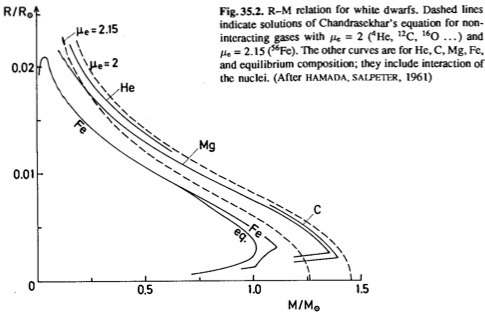
\includegraphics[width=(\textwidth-11mm),height=(\textheight-11mm),keepaspectratio]{M-R}
\caption{R-M relation for white dwarf: dashed lines indicate solution of Chandrasekhar equation for non-interacting gas with $\mu_e=2$ ($^4He$, $^{12}C$, $^{16}O$) and $\mu_e=2.15$ ($^{56}Fe$). The other are for He, C, Fe and equilibrium composition and include interactions with nuclei.}
\end{figure}


Trovo che esiste una massa limite per raggio tendente a zero e densit\'a infinita:
\begin{equation*}
M_{CSK}=M_3(R)=\frac{5.8\msun}{\mu_e^2}
\end{equation*}

\subsection{Chandrasekhar's limiting mass}

With increasing densities the electrons become gradually more relativistic: this start in the center where density is highest, the outer part remains non relativistic.

One can imagines an idealized model consisting of two regions fitted smoothly together: a relativistic polytrope core with $n=3$ surrounded by non-relativistci polytropic envelope with $n=\frac{3}{2}$.

At small mass the whole star is non-relativistic: the relativistic core will occur for $\rho_c\geq10^6\,gr/cm^3$.
For a polytrope of index $n=3$ the mass doesn't varies with central density:
\begin{align*}
M=4\pi (-\frac{w'}{z})|_{z_3}z_3^3(\frac{K}{\pi G})^{\frac{3}{2}}&\intertext{$\uparrow$ is called Chandrasekhar mass}\\
M_{Ch}=\frac{5.836}{\mu_e^2}\msun
\end{align*}

\section{Slowly rotating polytropes}

\subsection{Centrifugal acceleration from potential}

\begin{align*}
\Psi=\Phi+V&\intertext{con: }\\
\Phi=-\frac{GM}{r}\\
V=-\frac{1}{2}s^2\omega^2&\intertext{\'e possibile ricavare l'accelerazione centrifuga dal potenziale $\uparrow$. s \'e la distanza dall'asse di rotazione.}
\end{align*}

\subsection{Poisson equation for total potential}

Faccio la sostituzione $\Phi\to\Psi$: $\rho=[\frac{-\Psi}{(n+1)K}]^n
$.
\begin{align*}
\nabla^2\Psi=4\pi G\rho-2\omega^2\\
=4\pi G[\frac{-\psi}{(n+1)K}]^n-2\omega^2&\intertext{$\uparrow$ in coordinate adimensionali $y=Ar$ diventa:}\\
\Laplace_yw=w^n-\frac{\omega^2}{2\pi G\rho_c}\\
=w^n-\chi&\intertext{$\uparrow$ ho definito $\chi=\frac{\omega}{2\pi G\rho_c}$.}
\end{align*}

\subsection{Slow rotation approximation}

For $\chi\ll1$ I can approximate the solution $w(y,\theta)$ by expansion in Legendre polynomials $L_i(\theta)$:
\begin{align*}
w=w_0(y)+\chi w_1(y)+\chi w_2(y)L_2(\cos{\theta})+\ldots
\end{align*}


\chapter{Strutture autogravitanti in equilibrio: stabilit\'a rispetto a perturbazioni.}
\PartialToc


\section{Adiabatic processes: an approximation based upon physical consideration (time-scale)}

\subsection{Adiabatic evolution }
Short time-scale: adiabatic processes.
integration of equation under adiabatic condition
Properties of stellar interior under adiabatic condition

\subsection{Adiabatic exponent}

\begin{align*}
&\gamma_{ad}=\Dcvar{\PDly{\rho}{P}}{ad}&\intertext{se $\gamma_{ad}$ \'e costante, per trasformazioni adiabatiche, ho:}\\
&P\propto\rho^{\gamma_{ad}}
\end{align*}

Related to dynamical stability.

\subsection{Adiabatic temperature gradient}

\begin{align*}
&\nad=\Dcvar{\PDly{P}{T}}{ad}&\intertext{se $\nad$ \'e costante:}\\
&T\propto P^{\nad}
\end{align*}

Adiabatic temperature gradient is related to stability against convection.


\section{T. del viriale}

Chiamo U l'energia potenziale gravitazionale.

\subsection{Pressione nulla alla superficie}

\begin{align*}
&\sum_i\frac{1}{2}m_i\dvec{q_i}^2=\TDof{t}\sum_1\frac{1}{2}\vec{q_i}\dvec{q_i}-\sum_i\frac{1}{2}m_i\vec{q_i}\ddvec{q_i}&\intertext{quindi ho la prima formulazione del T  del viriale:}\\
&2E_{Kin}+U=\ddot{I}&\intertext{$\uparrow$ ho usato:}\\
&I=\sum_im_i\vec{q_i}^2\quad\ddot{I}=\TDof{t}(\sum_im_i\vec{q_i}\dvec{q_i})\\
&\sum_im_i\vec{q_i}\ddvec{q_i}=-\sum_i\vec{q_i}\nabla U=U & \intertext{$\uparrow$ sto gi\'a considerando un gas perfetto autogravitante. Se la velocit\'a e le dimensioni restano finite \'e possibile fare una media temporale:}\\
&\exv{2E_{Kin}+U}=0
\end{align*}

\subsection{Pressione esterna costante}

\begin{align*}
&\exv{2E_{Kin}+U-3PV}=0&\intertext{$\uparrow$ deriva da:}\\
&\sum_i\frac{1}{2}m_i\vec{q_i}\ddvec{q_i}\\
&=-U+\oint P\scap{r}{d\sigma}=-U+P\int_V(\scap{\nabla}{r})\,dV=\\
&-U+3PV
\end{align*}


\subsection{Pressione non omogenea}

\begin{align*}
&\exv{E_{Kin}}=\frac{3}{2}\exv{\int P\,dV}&\intertext{$\uparrow$ deriva da:}\\
&\sum_i\frac{1}{2}m_i\vec{q_i}\ddvec{q_i}=-U+\sum_i\oint_{\delta\sigma_i} P_i\scap{r_i}{d\sigma_i}\\
&=-U+\sum_i\int_{\delta V_i}\nabla(P_i\vec{r_i})\,dV_i\\
&=-U+3\int_VP\,dV+\sum_i\int_{\delta V_i}\scap{r_i}{g_i}\rho_i\,dV_i\\
&=-U+3\int_VP\,dV+\int_M\vec{r}\cdot(-\nabla\Phi)\,dm\\
&=3\int_VP\,dV
\end{align*}

Per pressione esterna nulla ho
\begin{equation*}
\exv{U}=-3\exv{\int P\,dV}
\end{equation*}


\section{Energia interna per stelle politrope. Generalizzazione del teorema del viriale.}

\subsection{Stella politropa}

\begin{align*}
&P=K\rho^{\frac{n+1}{n}}\\
&\TDy{r}{P}=-\frac{Gm(r)}{r^2}\rho(r)=-g(r)\rho(r)\\
&\PDy{r}{m}=4\pi r^2\rho(r)&\intertext{ $\uparrow$ ipotesi.}\\
&U=-G\int_0^Mm(r)\frac{\,dm}{r}\\
&=-\frac{GM^2}{2R}-G\int_0^R\frac{m^2(r)}{2r^2}\,dr&\intertext{Usando $\frac{dP}{\rho}=(n+1)d(\frac{P}{\rho})$:}\\
&U=-\frac{GM^2}{2R}+\frac{n+1}{2}\int m(r)\,d(\frac{P}{\rho})\\
&=-\frac{GM^2}{2R}+\frac{n+1}{2}\overbrace{\int_0^M\,d(\frac{mP}{\rho})}^{\approx0,\quad\frac{P}{\rho}\propto T}\\
&-\frac{n+1}{2}\int_0^M\frac{P}{\rho}\,dm&\intertext{Ho quindi:}\\
&U=-\frac{GM^2}{2R}-\frac{n+1}{2}\int P\,dV\\
&=-\frac{GM^2}{2R}+\frac{n+1}{6}U&\intertext{L'energia potenziale gravitazionale \'e:}\\
&U=-\frac{3}{5-n}\frac{GM^2}{R}
\end{align*}

\begin{comment}
\begin{tikzpicture}[overlay, remember picture]
\draw [decoration={brace,amplitude=0.5em,mirror},decorate,ultra thick,red] (first.north) -- (second.south) node[midway,label={[label distance=1mm]-100:Ipotesi}] {};
\end{tikzpicture}
\end{comment}
\index{Re-use: Tikzmark}

\subsection{Calcolo energia interna: stella politropa adiabatica.}

Densit\'a di energia interna.
\begin{align*}
&P=\alpha\rho^{1+\frac{1}{n_{AD}}}&\intertext{Esplicito la dipendenza dell'energia interna da $P$ e $\rho$ usando la condizione di adiabaticit\'a:}\\
&(dE+P\,dV=0,\ V=Mv=\frac{M}{\rho},\  E=e_IM)\\
&e_I\propto\rho^{\delta}P^{\xi}=\beta\rho^{\theta}\\
&(P=-\left.\frac{\partial E}{\partial V} \right|_{S,A}=-\frac{\partial (\frac{E}{A})}{\partial (\frac{V}{A})}\\
&=-\frac{\partial \epsilon}{\partial \frac{1}{\rho}}=\rho^2 \frac{\partial \epsilon}{\partial \rho})\\
&P=-(\PDy{V}{E})_S\xrightarrow{\rho=\frac{1}{v}}\rho^2(\TDy{\rho}{e_I})_S=\theta\beta\rho^{\theta+1}&\intertext{quindi ricavo gli esponenti:}\\
&\theta_{AD}=\frac{1}{n_{AD}}\quad\beta=\frac{\alpha}{\theta}=\alpha n_{AD}&\intertext{Gas perfetto monoatomico $\downarrow$}\\
&n_{AD}=\frac{3}{2}&\intertext{Gas di radiazione $\downarrow$}
&n_{AD}=3\\
&e_I=n_{AD}\frac{P}{\rho}
\end{align*}

\subsection{Generalizzazione del teorema del viriale: tengo conto dell'energia interna (solo termica).}

\begin{align*}
&\int P\,dV=\frac{1}{n_{Ad}}\int e_I\rho\,dV\\
&=\frac{1}{n_{Ad}}\int e_i\,dM=\frac{1}{n_{Ad}}E_{Int}&\intertext{$\uparrow$ ho integrato $e_I=n_{Ad}\frac{P}{\rho}$ in $dV$. Utilizzando:}\\
&\exv{U}=-3\int P\,dV&\intertext{ottengo}\\
&E_{Int}=-\frac{n_{Ad}}{3}U
\end{align*}

Infine ho una relazione fra l'energia totale $E$ e l'energia potenziale gravitazionale (dipendente dall'indice adiabatico e da quello politropico) se $\xi=3\frac{\rho}{P}\TDy{\rho}{P}-3=3(\gamma_{Ad}-1)$ \'e costante in tutta la stella:
\begin{align*}
&E=E_{Int}+U=\frac{3-n_{Ad}}{3}U=\frac{3-n_{Ad}}{5-n}\frac{GM^2}{R}&\intertext{ che nel caso di una struttura convettiva ($n=n_{Ad}$) diventa:}\\
&E=-\frac{3}{7}\frac{GM^2}{R}
\end{align*}



\section{Criterio di stabilit\'a}

\subsection{Perturbazione adiabatica}

Perturbazione self-similar: \mblock{r\to r+\delta r=(1+\alpha)r}.
\begin{align*}
&v=\frac{1}{\rho}\to(1+\alpha)^3v,\quad\,dv\to(1+\alpha)^3\,dv&\intertext{quindi al secondo ordine in $\alpha$ ho:}\\
&\delta v=(3\alpha+3\alpha^2)v,\quad (\delta v)^2=(3\alpha)^2v^2,\\
&\rho\to(1+\alpha)^{-3}\rho,\\
&M\to M\\
&-P=\PDy{v}{e_I}&\intertext{$\uparrow$ primo principio $dq=/,du+P\,dv$ per trasformazioni adiabatiche}\\
&\gamma_{Ad}\frac{P}{v}=-\Dcvar{\PDy{v}{P}}{Ad}=\Dcvar{\TtwoDy{v}{e_I}}{Ad}&\intertext{La prima ugaglianza di $\uparrow$ deriva dalla definizione di $\gamma_{Ad}=\Gamma_{Ad}=\Dcvar{\TDly{\rho}{P}}{Ad}$, la secando uguaglianza dalla sostituzione della prima equazione.}
\end{align*}

Determino la variazione di energia al secondo ordine in $\alpha$:
\begin{align*}
&E=\int\,dM[e_I-\frac{GM(r)}{r}]\\
&e_I\to e_i+\Dcvar{\PDy{v}{e_I}}{Ad}\delta +\frac{1}{2}\Dcvar{\PtwoDy{v}{e_i}}{Ad}(\delta v)^2&\intertext{$\uparrow$ primo principio}\\
&\approx e_I-Pv(3\alpha+3\alpha^2)\\
&+\frac{1}{2}\Gamma_{Ad}\frac{P}{v}(3\alpha)^2v^2&\intertext{da cui:}\\
&E=\int\,dM[e_I-Pv(3\alpha+3\alpha^2)\\
&+\frac{1}{2}\Gamma_{Ad}\frac{P}{v}(3\alpha)^2v^2\\
&-\frac{1}{1+\alpha}\frac{GM}{r}]\\
&\delta E=\int\,dV[\alpha(-3P+\frac{GM(r)}{r}\rho)\\
&+\alpha^2(-3P+\frac{9}{2}\Gamma_{Ad}P-\frac{GM(r)}{r}\rho)]
\end{align*}


\subsection{Condizione di stabilit\'a}

La condizione di equilibrio \'e data dall'annullarsi del coefficiente lineare in $\alpha$:
\begin{equation*}
3\int\,dV=\int\frac{Gm(r)\rho}{r}\,dV=-U
\end{equation*}
La condizione di stabilit\'a \'e data dalla positivit\'a della derivata seconda
\begin{align*}
&\int\,dV[-3P+\frac{9}{2}\Gamma_{Ad}P-\frac{GM\rho}{r}]>0\\
&\int(\Gamma_{Ad}-\frac{4}{3})P\,dV>0
\end{align*}

\subsection{Perturbazione di ampiezza finita}

Dipendenza della pressione dalla densit\'a in condizioni di equilibrio
\begin{align*}
&P\propto GM^{\frac{2}{3}}\overline{\rho}^{\frac{4}{3}}(R)&\intertext{$\uparrow$ ricavata da:}\\
&Const\,GM^{\frac{2}{3}}\overline{\rho}^{\frac{4}{3}}(R)\leq P_c\leq\,Const\,GM^{\frac{2}{3}}\rho_c^{\frac{4}{3}}\\
&\frac{\delta P}{P}=\frac{4}{3}\frac{\delta\rho}{\rho}
\end{align*}

Perturbazione Adiabatica:
\begin{align*}
&\frac{\delta P}{P}=\Gamma_{Ad}\frac{\delta\rho}{\rho}\\
&P=P_0(\frac{\rho}{\rho_0})^{\Gamma_{Ad}}&\intertext{$\Gamma_{Ad}$ costante, $(P_0,\rho_0)$ condizione di equilibrio, con:}\\
&P_0=AGM^{\frac{2}{3}}\rho_0^{\frac{4}{3}},\quad A\approx1 &\intertext{Descrivo una perturbazione adiabatica con:}\\
&P(\rho)=P_0(\frac{\rho}{\rho_0})^{\Gamma_{Ad}}=(1-F)AGM^{\frac{2}{3}}(\frac{\rho}{\rho_0})^{\frac{4}{3}}\rho_0^{\frac{4}{3}}&\intertext{dalla condizione di equilibrio ho:}\\
&P(\rho)=(1-F)(\frac{\rho}{\rho_0})^{\frac{4}{3}}P_0&\intertext{confrontando le due equazioni ricavo:}\\
&1-F=(\frac{\rho}{\rho_0})^{\Gamma_{Ad}-\frac{4}{3}}&\intertext{se a causa di una perturbazione ho $\rho>\rho_0$, $\uparrow$ implica}\\
&\intertext{Per $\Gamma_{Ad}>\frac{4}{3}$, la densit\'a tende verso il valore di equilibrio. Ho l'equazione del moto radiale per un guscio sferico:}\\
&\TtwoDy{t}{r}=-F\frac{Gm(r)}{r^2}>0&\intertext{$\uparrow$ perch\'e $F<0(1-F>1)$.}\\
&\intertext{Per $\Gamma_{Ad}<\frac{4}{3}$, la densit\'a diverge dal valore di equilibrio. Ho l'equazione del moto radiale per un guscio sferico:}\\
&\TtwoDy{t}{r}=-F\frac{Gm(r)}{r^2}<0&\intertext{$\uparrow$ perch\'e $F>0(1-F<1)$.}
\end{align*}

Per $\Gamma_{Ad}>\frac{4}{3}$ la pressione cresce/diminuisce troppo rapidamente all'aumentare/diminuire di $\rho$ bloccando la contrazione/espansione.

Per $\Gamma_{Ad}>\frac{4}{3}$ la perturbazione \'e destinata a crescere.

\section{Problema delle pulsazioni.}


\subsection{Pulsazioni radiali: modello elementare}
vedi cox

\subsection{Effetto della perturbazione sull'energia: secondo ordine.}

Per $\Gamma_{Ad}<\frac{4}{3}$ una perturbazione pu\'o essere amplificata esponenzialmente 
\begin{align*}
&v\to(1+\alpha)^3v,\quad \frac{\delta r}{r}=\frac{\delta R}{R}=\alpha\\
&E=\int\,dm[e_I-\frac{Gm(r)}{r}]\\
&\delta E\approx\alpha^2\underbrace{\int\,dV(-3P+\frac{9}{2}\Gamma_{Ad}P-\frac{Gm(r)\rho}{r})}_{=\frac{3}{2}\int\,dVP(3\Gamma_{Ad}P-4)=-\frac{U}{2}\exv{4\Gamma_{Ad}-4}}&\intertext{Posto $-U=\xi\frac{GM^2}{R}$, dove $\xi\approx1$, riscrivo}\\
&\delta E\approx\frac{1}{2}\xi\frac{GM^2}{R}\exv{(3\Gamma_1-4)(\frac{\delta r}{r})^2}
\end{align*}

\subsection{Periodo di pulsazione}

\begin{align*}
&\omega^2=\frac{K'}{M}=\xi G\frac{M}{R^3}\exv{3\Gamma_1-4}\\
&=\frac{4}{3}\xi\pi G\overline{\rho}\exv{3\Gamma_1-4}\\
&\tau_{Puls}=\frac{2\pi}{\omega}\approx t_{ff}&\intertext{$\uparrow$ se $\exv{3\Gamma_1-4}$ \'e abbastanza lontano da zero.}
\end{align*}

\subsection{Relazione Periodo-Luminosit\'a}

\begin{align*}
&\frac{\tff}{\tkh}\approx\frac{\Pi}{\tkh}\approx\frac{LR^{\frac{5}{2}}}{G^{\frac{3}{2}}M^{\frac{5}{2}}}\approx\sci{-12}\frac{LR^{\frac{5}{2}}}{M^{\frac{5}{2}}}\\
&L\propto M^{\frac{2}{3}}T_e^4t_{puls}^{\frac{4}{3}}&\intertext{$\uparrow$ la temperatura effettiva \'e definita da:}\\
&L=4\pi R^2aT_e^4
\end{align*}

\subsection{Zone di ionizzazione parziale}

La teoria delle stelle pulsanti mette in evidenza l'importanza delle zone di ionizzazione parziale.




\chapter{Nane bianche}
\PartialToc

\section{Spectra of white dwarf}

Lines in spectra of white dwarf are strongly broadened by pressure effects: the wings of hydrogen lines overlap.

\subsection{Statistical Stark effect}

conditions under which hydrogen lines merge into the continuum, disappearance of higher quantum states and formation of continuus spectrum.

\section{Internal constitution}


\section{Physical properties of dense matter}

\end{document}